%%%%%%%%%%%%%%%%%%%%%%%%%%%%%%%%%%%%%%%%%
% Beamer Presentation
% LaTeX Template
% Version 1.0 (10/11/12)
%
% This template has been downloaded from:
% http://www.LaTeXTemplates.com
%
% License:
% CC BY-NC-SA 3.0 (http://creativecommons.org/licenses/by-nc-sa/3.0/)
%
%%%%%%%%%%%%%%%%%%%%%%%%%%%%%%%%%%%%%%%%%

%----------------------------------------------------------------------------------------
%	PACKAGES AND THEMES
%----------------------------------------------------------------------------------------

\documentclass{beamer}

\mode<presentation> {

% The Beamer class comes with a number of default slide themes
% which change the colors and layouts of slides. Below this is a list
% of all the themes, uncomment each in turn to see what they look like.

%\usetheme{default}
%\usetheme{AnnArbor}
%\usetheme{Antibes}
%\usetheme{Bergen}
%\usetheme{Berkeley}
%\usetheme{Berlin}
%\usetheme{Boadilla}
%\usetheme{CambridgeUS}
%\usetheme{Copenhagen}
%\usetheme{Darmstadt}
%\usetheme{Dresden}
%\usetheme{Frankfurt}
%\usetheme{Goettingen}
%\usetheme{Hannover}
%\usetheme{Ilmenau}
%\usetheme{JuanLesPins}
%\usetheme{Luebeck}
\usetheme{Madrid}
%\usetheme{Malmoe}
%\usetheme{Marburg}
%\usetheme{Montpellier}
%\usetheme{PaloAlto}
%\usetheme{Pittsburgh}
%\usetheme{Rochester}
%\usetheme{Singapore}
%\usetheme{Szeged}
%\usetheme{Warsaw}

% As well as themes, the Beamer class has a number of color themes
% for any slide theme. Uncomment each of these in turn to see how it
% changes the colors of your current slide theme.

%\usecolortheme{albatross}
%\usecolortheme{beaver}
%\usecolortheme{beetle}
%\usecolortheme{crane}
%\usecolortheme{dolphin}
%\usecolortheme{dove}
%\usecolortheme{fly}
%\usecolortheme{lily}
%\usecolortheme{orchid}
%\usecolortheme{rose}
%\usecolortheme{seagull}
%\usecolortheme{seahorse}
%\usecolortheme{whale}
%\usecolortheme{wolverine}

%\setbeamertemplate{footline} % To remove the footer line in all slides uncomment this line
%\setbeamertemplate{footline}[page number] % To replace the footer line in all slides with a simple slide count uncomment this line

%\setbeamertemplate{navigation symbols}{} % To remove the navigation symbols from the bottom of all slides uncomment this line
}

\usepackage{graphicx} % Allows including images
\usepackage{booktabs} % Allows the use of \toprule, \midrule and \bottomrule in tables
\usepackage{multicol}
\usepackage{bbding}
\usepackage{color}
%\usepackage{cite}


%----------------------------------------------------------------------------------------
%	TITLE PAGE
%----------------------------------------------------------------------------------------

\title[]{Row Projection Algorithms} % The short title appears at the bottom of every slide, the full title is only on the title page

\author{Wei Deng,  Nicole Eikmeier, \\ Nate Veldt,  Xiaokai Yuan} % Your name
\institute[UCLA] % Your institution as it will appear on the bottom of every slide, may be shorthand to save space
{
Purdue University \\ % Your institution for the title page
\medskip
%\textit{john@smith.com} % Your email address
}
\date{\today} % Date, can be changed to a custom date

\begin{document}

\begin{frame}
\titlepage % Print the title page as the first slide
\end{frame}

%\begin{frame}
%\frametitle{Overview} % Table of contents slide, comment this block out to remove it
%\tableofcontents % Throughout your presentation, if you choose to use \section{} and \subsection{} commands, these will automatically be printed on this slide as an overview of your presentation
%\end{frame}



%----------------------------------------------------------------------------------------
%	PRESENTATION SLIDES
%----------------------------------------------------------------------------------------

%------------------------------------------------
%------------------------------------------------
% FIRST SECTION
%------------------------------------------------
%------------------------------------------------

%\section{First Section} % Sections can be created in order to organize your presentation into discrete blocks, all sections and subsections are automatically printed in the table of contents as an overview of the talk
%------------------------------------------------

%\subsection{Subsection Example} % A subsection can be created just before a set of slides with a common theme to further break down your presentation into chunks

%\frame{
%\frametitle {Reverse Cuthill-Mckee}
%\begin{figure}[htbp] %  figure placement: here, top, bottom, or page
%   \centering
%   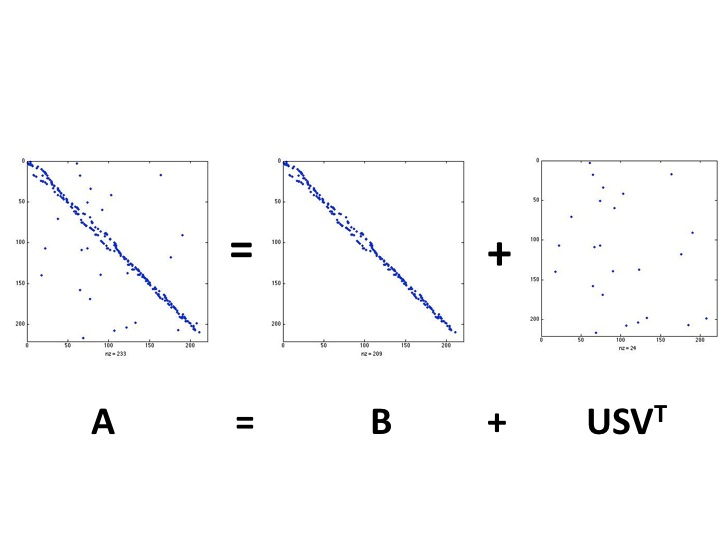
\includegraphics[width=4in]{Project4Pics/Slide1.jpg}
%   \caption{example caption}
%   \label{fig:example}
%\end{figure}
%}


\frame
{
  \frametitle{Problem Setup}
We seek solutions to:

\[ \bf{ Ax = f} \]

\begin{itemize}
\item $A$ is large, sparse, and may not be symmetric
\item $A$ can undergo a symmetric permutation to become banded
\end{itemize}

}


%------------------------------------------------
%------------------------------------------------
% Wei's Part

\frame{
\frametitle{Kaczmarz method}

Finding a common point of a set of hyperplanes $S_i=\{x:A_ix-b_i=0\}$ for $i=1,2,...$, where $A_i$ and $b_i$ are $i$th row of matrix $A$ and vector $b$\\

\begin{figure}[htbp]
\begin{minipage}[b]{0.8\linewidth}
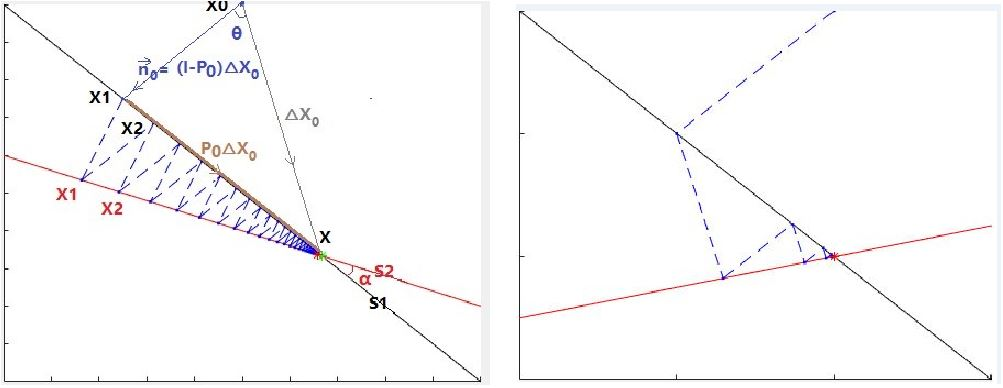
\includegraphics[width=3.5in]{Images/Classical_Kaczmarz}
\caption{2-Partition Case}
\end{minipage}
\end{figure}

So, the classical Kaczmarz method: $x_k=x_k+\overrightarrow{n_k}=x_k+\frac{r_k^i}{||A_i||^2}A_i^T$\\
where  $\overrightarrow{n_k}=\bigtriangleup{x_k}cos\theta=\frac{\langle\,A_i{,}\,\bigtriangleup{x_k}\rangle}{||A_i||^2}A_i^T=\frac{b_i-\langle\,A_i{,}\,x_k\rangle}{||A_i||^2}A_i^T=\frac{r_k^i}{||A_i||^2}A_i^T$\\
}




\frame{
\frametitle{Block Gauss-Seidel}

\begin{figure}[htbp]
\begin{minipage}[b]{0.8\linewidth}
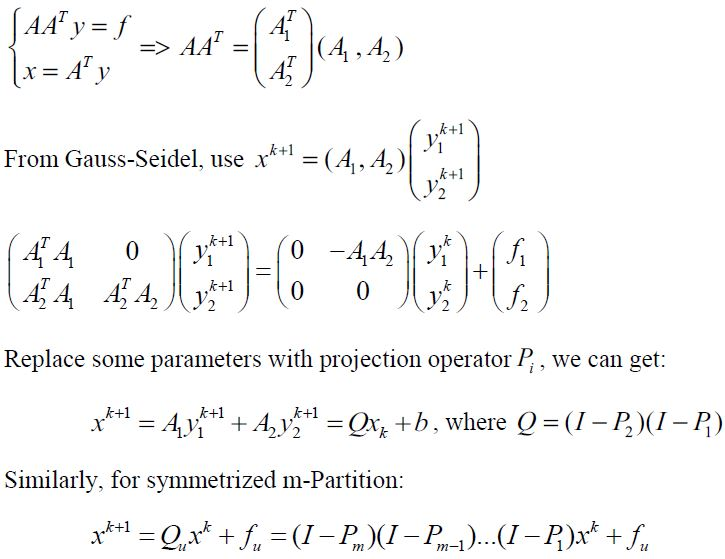
\includegraphics[width=3.5in]{Images/Gauss-Seidel}
\end{minipage}
\end{figure}
}

\frame{
\frametitle{Symmetrization and Acceleration}

\begin{figure}[htbp]
\begin{minipage}[b]{0.9\linewidth}
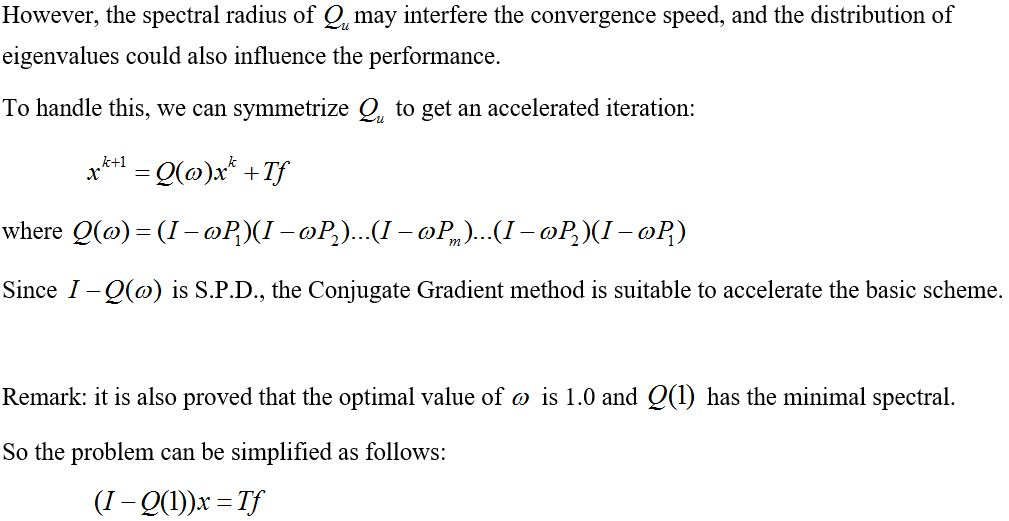
\includegraphics[width=4.5in]{Images/Symmetrize-Q}
\end{minipage}
\end{figure}
}


\frame{
\frametitle{Permutation}

\begin{figure}[htbp]
\begin{minipage}[b]{0.7\linewidth}
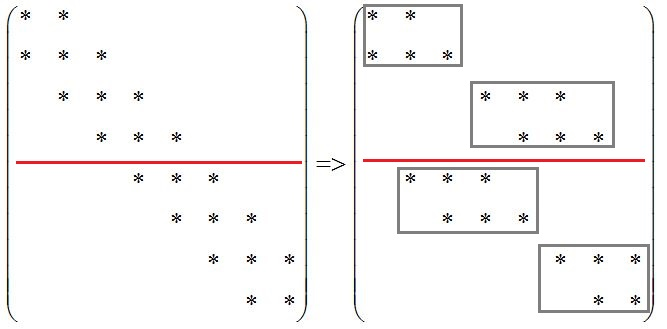
\includegraphics[width=3.5in]{Images/permutation}
\end{minipage}
\end{figure}

}

%------------------------------------------------
%------------------------------------------------






\frame{
\frametitle{Reverse Cuthill-Mckee}

We can perform a symmetric permutation with matrix $P$:
\begin{figure}[ht]
\centering
\begin{minipage}[b]{0.45\linewidth}
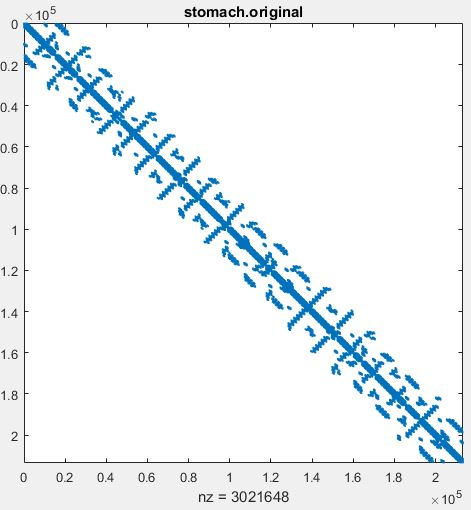
\includegraphics[width=2in]{Images/SparseA_v5.jpg}
\caption{$A$ sparse, non-symmetric}

\end{minipage}
\quad
\begin{minipage}[b]{0.45\linewidth}
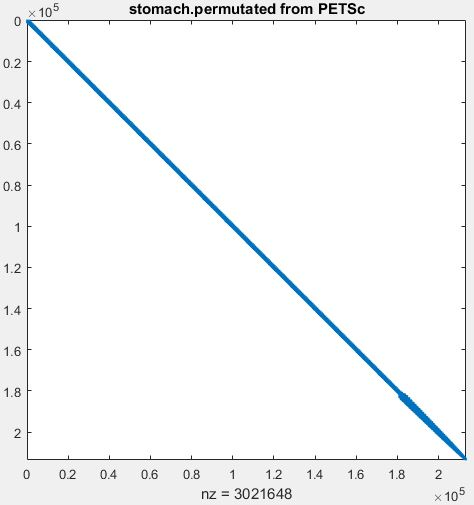
\includegraphics[width=2in]{Images/Arcm_v3.jpg}
\caption{$P^TAP$ (banded)}

\end{minipage}
\end{figure}

}

\frame{
\frametitle{If Bandwidth Too Large}

For some problems the bandwidth could be too large, so instead we could choose $P$ so that:

\begin{figure}[ht]
\centering
\begin{minipage}[b]{0.45\linewidth}
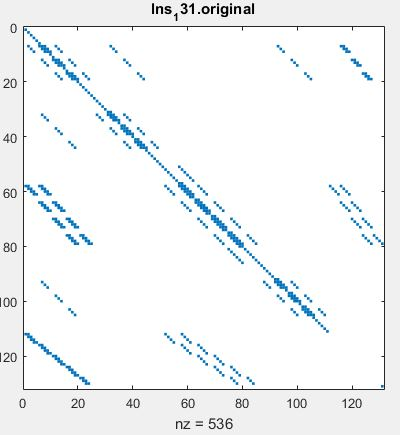
\includegraphics[width=1.7in]{Images/SparseA_v4.jpg}
\caption{$A$ is sparse and non-symmetric}

\end{minipage}
\quad
\begin{minipage}[b]{0.45\linewidth}
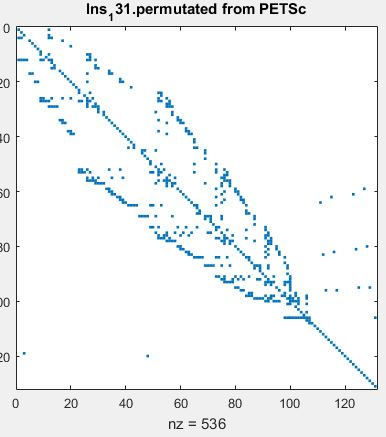
\includegraphics[width=1.7in]{Images/ApproxBanded_v2.jpg}
\caption{$P^TAP$ narrow band+low rank}

\end{minipage}
\end{figure}

}




\frame{
\frametitle{narrow band+low rank }
\begin{figure}[htbp] %  figure placement: here, top, bottom, or page
   \centering
   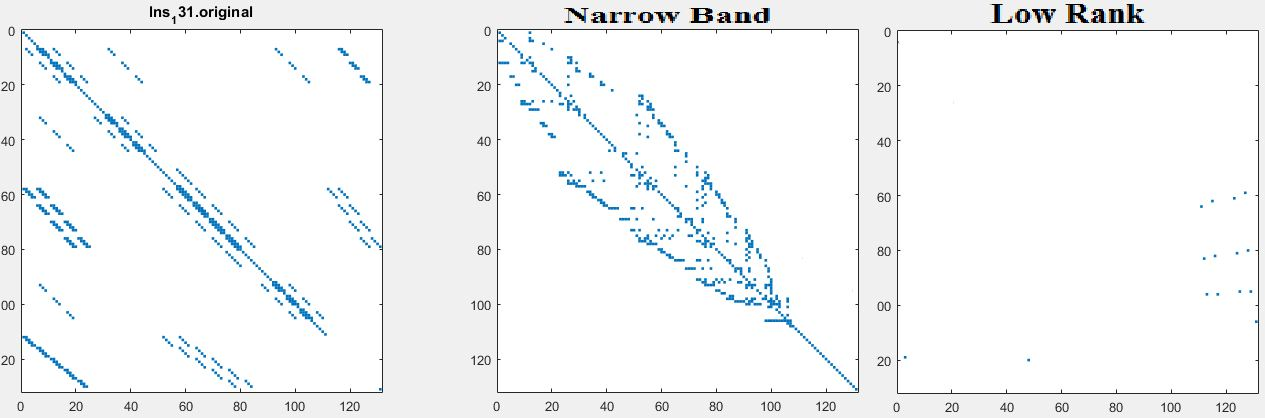
\includegraphics[width=4.5in]{Images/BandLowRank.jpg}
   \caption{Breaking up $A$ into a banded matrix plus a low rank matrix}
\end{figure}
}

\frame{
\frametitle{Woodbury Formula}
To solve
$$ Ax = b \implies x = A^{-1} b$$
we use the following formula:
\begin{block}{Woodbury Formula}
\begin{align*}
A^{-1} &= (B - USV^T)^{-1}\\
	  &= B^{-1} - B^{-1}UTV^TB^{-1}
\end{align*}
where $T = (V^TB^{-1}U - S^{-1})^{-1}$
\end{block}
}

\frame{
\frametitle{Solving $Ax = b$}
Solving system:
\begin{align*}
x &= A^{-1}b\\
   &= {\bf B^{-1} b} - B^{-1}UTV^T {\bf B^{-1} b} \\
   &= {\bf a} - B^{-1}UT(V^T {\bf a}) \\
   &= {\bf a} - B^{-1}UT {\bf c}  \hspace{.5cm} \mbox{( solve ($V^TB^{-1}U-S^{-1}) \textbf{d} = \textbf{c}$)}\\
   &= {\bf a} - B^{-1}U\textbf{d}\\
   &= {\bf a} - B^{-1}\textbf{h}
\end{align*}

All systems involving $B$ are relatively easy to solve. \newline

Alternatively, we could just get $B$ and use it as a preconditioned for a Krylov subspace method.

}




%%%%%%%%%%%%%%%


\begin{frame}
\frametitle{Bandwidth after RCM reordering}

Let's see the performance after the Reverse Cuthill Mckee

\begin{center}
\begin{tabular}{| l | l | c  c  c}
\hline

    matrix           & size         &    Matlab & PETSc     &  rcm.cpp        \\
 \hline
 lns                   & 131             &     32        &       \color{red} $\times$ 111         & \color{red} $\times$ 113  \\
 ac2-db            & 21,982     &         545       &     \color{red} $\times$            &  \color{red} $\times$  \\
 bayer01           & 57,735      &     \color{red} $\times$ 18,322        &     \color{red} $\times$     &  \color{red} $\times$   \\
 venkat25         & 62,424      &     1,515        &    1,515    & 1,495                   \\
 stomach          & 213,360    &      1,133      & 2,216 & 2,239                    \\
 atmosmodd     & 1,270,432 &    7,772       & 7,772&  7,772                   \\
 \hline

\end{tabular}
\end{center}


\end{frame}


\frame{
\frametitle{Re-ordering}

To make the matrix better for parallelism, we do the following permutation

\begin{figure}[ht]
\centering
\begin{minipage}[b]{1.0\linewidth}
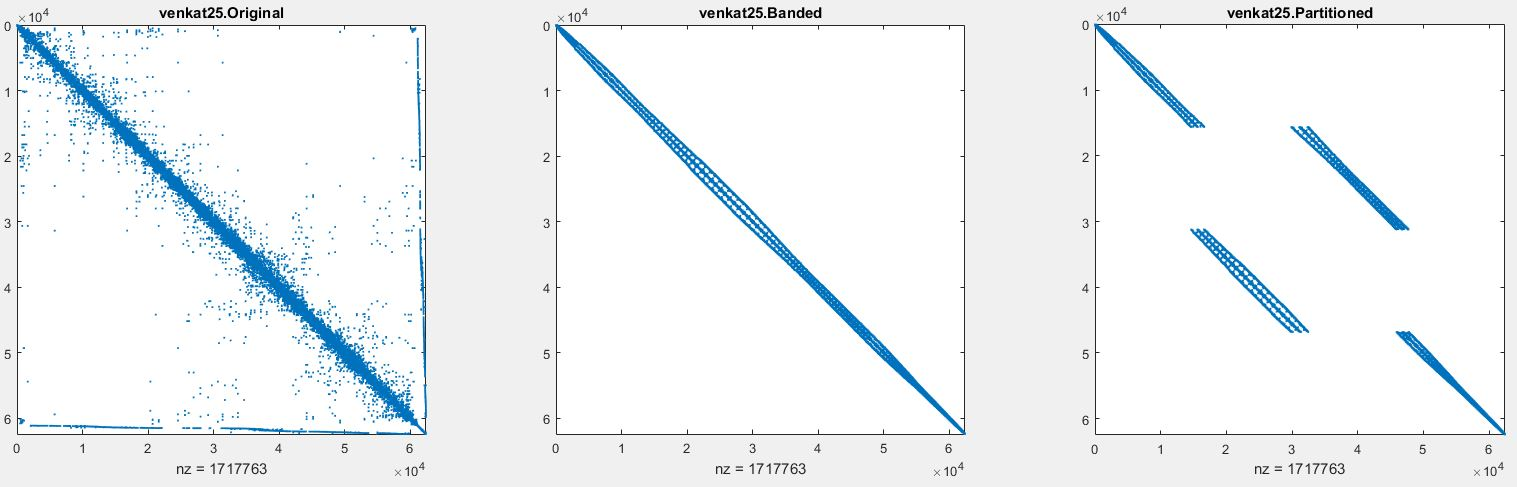
\includegraphics[width=4.8in]{Images/permute.jpg}
\caption{$A$ is partitioned into 2 parts with several independent submatrices}

\end{minipage}
\end{figure}

}


\frame{
\frametitle{Quality of Re-ordering}

The test cases show that, 2 partion has the best performance, and with the number of blocks in each partition increasing, the performance goes better.

\begin{figure}[ht]
\centering
\begin{minipage}[b]{1\linewidth}
\includegraphics[width=4.5in]{Images/quality.jpg}

\end{minipage}
\end{figure}

}





%------------------------------------------------
%------------------------------------------------
% THIRD SECTION
%------------------------------------------------
%------------------------------------------------

%------------------------------------------------
%------------------------------------------------
% NATE'S SLIDES FOR FINAL PRESENTATION ON THURSDAY
%------------------------------------------------
%------------------------------------------------
\begin{frame}
\frametitle{New System After Permutation}

\begin{block}{Original non-symmetric system}
$${\bf A x = f}$$
$A$ is large, sparse, and non-symmetric
\end{block}


\begin{block}{New Symmetric Positive Definite System}

$${\bf (I-Q)x = c} $$

where
$$Q = (I-P_1)(I-P_2) \cdots (I-P_m) \cdots (I-P_1),$$
 $$P_i = A_i(A_i^TA_i)^{-1}A_i^T$$
 $$ c = A^{T}(D+L)^{-T}D(D+L)^{-1}f $$
\end{block}
\end{frame}


\begin{frame}
\frametitle{Computing c = Tf}

%For our code we assume two partitions:
%
$$A = \begin{bmatrix} A_1^T  \\ A_2^T \end{bmatrix}, \hspace{.1cm} f = \begin{bmatrix} f_1  \\ f_2 \end{bmatrix}$$
\begin{figure}[htbp] %  figure placement: here, top, bottom, or page
   \centering
   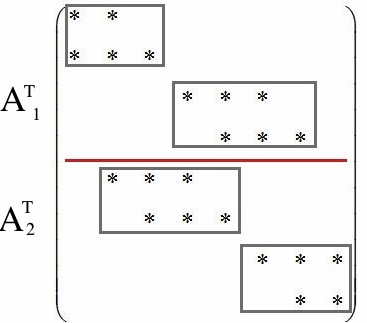
\includegraphics[width=2in]{Images/A1A2.jpg}
\end{figure}
\end{frame}

\begin{frame}
\frametitle{Computing c = Tf}

$$\textbf{Tf} = \begin{bmatrix} (I + (I-P_2)(I-P_1))(A_1^T)^+ && (I-P_1)(A_2^T)^+ \end{bmatrix} \begin{bmatrix} f_1  \\ f_2 \end{bmatrix}= c $$

\begin{enumerate}
\item Solve pseudo-inverse problem:
$$v_i = (A_i^T)^+f_i$$
\item Perform least squares computations of the form:
$$ (I-P_i) x =  y$$
\end{enumerate}
\end{frame}






\begin{frame}
\frametitle{Conjugate Gradient Method (Kamath and Sameh, 1988) }
\textbf{Step 1} : $x_0 = c$ \\
\hspace{.5in} Compute $r_0 = Tf - (I-Q)c = Qc$\\
\hspace{.5in} Set $p_0 = r_0, i = 0$ \\
\textbf{Step 2}:  Compute: \\
\hspace{.5in} $\alpha_i = (r_i, r_i)/(p_i, (I-Q)p_i)$ \\
\hspace{.5in} $ x_{i+1} = x_i + \alpha_i p_i $ \\
\hspace{.5in} $\beta_i = (r_{i+1}, r_{i+1})/(r_i, r_i) $ \\
\hspace{.5in} $p_{i+1} = r_{i+1} + \beta_i p _i $ \\
\textbf{Step 3}: If convergence criterion is satisfied, terminate the iterations; else set $i = i+1$ and return to Step 2.

\vspace{.4in}
%We can take a convergence criterion as : $$ \frac{ ||f - A x_i ||}{|| f - A x_0 || } \leq 10^{-6} $$
 We can take a convergence criterion as : $$ \frac{ ||r_i||}{||r_0||} \leq \epsilon$$
\end{frame}


\begin{frame}
\frametitle{Key Step in the Framework is Least Squares Computations }
\textbf{Step 1} : $x_0 = c$ \\
\hspace{.5in} Compute $r_0 = Tf - \boxed{(I-Q)c} = Qc$\\
\hspace{.5in} Set $p_0 = r_0, i = 0$ \\
\textbf{Step 2}:  Compute: \\
\hspace{.5in} $\alpha_i = (r_i, r_i)/(p_i,\boxed{(I-Q)p_i})$ \\
\hspace{.5in} $ x_{i+1} = x_i + \alpha_i p_i $ \\
\hspace{.5in} $\beta_i = (r_{i+1}, r_{i+1})/(r_i, r_i) $ \\
\hspace{.5in} $p_{i+1} = r_{i+1} + \beta_i p _i $ \\
\textbf{Step 3}: If convergence criterion is satisfied, terminate the iterations; else set $i = i+1$ and return to Step 2.

\vspace{.4in}
%We can take a convergence criterion as : $$ \frac{ ||f - A x_i ||}{|| f - A x_0 || } \leq 10^{-6} $$
 We can take a convergence criterion as : $$ \frac{ ||r_i||}{||r_0||} \leq \epsilon$$
\end{frame}




%------------------------------------------------
%------------------------------------------------
% Xiaokai Yuan
%%%%%%%%%%%%%%%%%%%%%%%%%%%%%%%%%%%%%%%%%%%%%%%%%%%%%%%%%%%%%%%%%%%%%%%%%%%%%%%%%%%%%%%%%%%%%%%%%%%%%%%%%%%%%%%%%%%%%%%%%%%%%
\begin{frame}
 \frametitle{Compute $x_{k}=(I-P_{i})x_{k}$}
 \begin{itemize}
  \item It is not stable to form $P_{i}$ directly since it will double the condition number of $A_{i}$, and at the same time will cost time on solving
        $(A^{T}_{i}A_{i})^{-1}$.
  \item Given a vector $u$ obtain $v=(I-P_{j})u \Leftrightarrow \min\limits_{v}||u-A_{j}w||_{2}$.
  \item Solve $\min\limits_{v}||u-A_{j}w||_{2}$ directly: Normal equation is unstable, QR decomposition and SVD decomposition are too slow.
  \item Petsc: using CG method on normal equation: $A_{j}^{T}A_{j}w=A_{j}^{T}u$.
  \item Parallel step:
        \begin{equation*}
            \begin{split}
                v&=\min\limits_{v}||u-A_{j}w||_{2}\Leftrightarrow \min\limits_{v_{i}}||u_{i}-A_{j,i}w_{i}||_{2},\\
                v&^{T}=[v_{1}^{T},v_{2}^{T},...,v_{k}^{T}],\\
                w&^{T}=[w_{1}^{T},w_{2}^{T},...,w_{k}^{T}].
            \end{split}
        \end{equation*}
 \end{itemize}


\end{frame}


\begin{frame}
\frametitle{QR factorization for $Ax=b$}
\begin{itemize}
  \item $A_{m,n}$.
  \item $A=QR,\quad and\quad Rx=Q^{T}b$.
  \item QR factorization of A needs: $2mn^2 \quad flops$.
  \item form $d=Q^{T}b$ needs: $2mn \quad flops$.
  \item Solve $Rx=d$ by back substitution: $n^2 \quad flops$.
  \item for large $m, n$, the cost is about $2mn^2$.
\end{itemize}
\end{frame}

\begin{frame}
\frametitle{Cholesky factorization for $A^{T}Ax=A^{T}b$}
\begin{itemize}
    \item calculate $C = A^{T}A :2n(n + 1)(2m - 1) \approx mn^{2}$ flops.
    \item Cholesky factorization $C = LL^{T}: \frac{1}{3}n^{3}$ flops.
    \item calculate $d = A^{T}b :2mn$ flops.
    \item solve Lz = d by forward substitution :$n^2$ flops.
    \item solve $L^{T}x = z$ by back substitution :$n^2$ flops.
    \item cost for large $m, n: mn^{2} + \frac{1}{3}n^3$ flops
\end{itemize}
\end{frame}

\begin{frame}
\frametitle{sensitive of $A~p_{k}$}
\begin{itemize}
    \item $x=ones(m,1),A_{m,m}, eig(A)\in (0,1), m=1000, tolerance=10^{-8}$.
\end{itemize}

\begin{figure}[htbp]
\begin{minipage}[b]{0.8\linewidth}
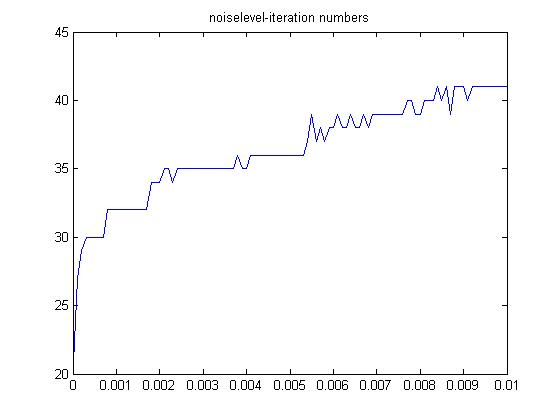
\includegraphics[width=3.5in]{Images/noiselevel_iteration}
\end{minipage}
\end{figure}
\end{frame}

\begin{frame}
\begin{figure}[htbp]
\begin{minipage}[b]{0.8\linewidth}
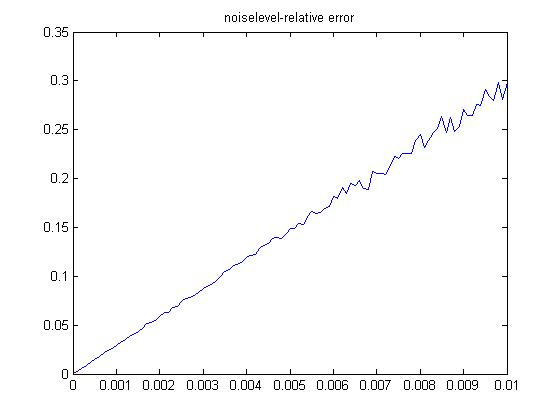
\includegraphics[width=3.5in]{Images/noiselevel_relativeerror}
\end{minipage}
\end{figure}

\end{frame}


\begin{frame}
\frametitle{LSQR and Lanczos process}
\begin{itemize}
    \item LSQR: An Algorithm for Sparse Linear Equations and Sparse Least Squares, Christopher C.Paige, Michael A. Saunders.
    \item Step1, $\beta_{1}u_{1}=b, \alpha_{1}v_{1}=A^{T}u_{1}, w_{1}=v_{1}, x_{0}=0, \bar{\phi_{1}}=\beta_{1},\bar{\rho_{1}}=\alpha_{1}$.\\
                 needs $2mn$ flop.
    \item Step2, bidiagonalization needs $4mn$ flop.
    \item       $\quad a.\beta_{i+1}u_{i+1}=Av_{i}-\alpha_{i}u_{i}$.
    \item       $\quad b.\alpha_{i+1}v_{i+1}=A^{T}u_{i+1}-\beta_{i+1}v_{i}$.
\end{itemize}
\end{frame}

\begin{frame}
\begin{itemize}
    \item Step3, orthogonal transformation
    \item       $\quad a.\rho_{i}=\sqrt{(\bar{\rho_{i}^2}+beta_{i+1}^2)}$,
    \item       $\quad b.c_{i}=\bar{\rho_{i}}/\rho_{i},$
    \item       $\quad c.s_{i}=\beta_{i+1}/\rho_{i},$
    \item       $\quad d.\theta_{i+1}=s_{i}\alpha_{i+1},$
    \item       $\quad e.\bar{\rho_{i+1}}=-c_{i}\alpha_{i+1},$
    \item       $\quad f.\phi_{i}=c_{i}\bar{\phi_{i}},$
    \item       $\quad g.\bar{\phi_{i+1}}=s_{i}\bar{\phi_{i}}.$
    \item Step4, Update x, w need $4n$ flop.
    \item       $\quad a.x_{i}=x_{i-1}+(\phi_{i}/\rho_{i})w_{i},$
    \item       $\quad b.w_{i+1}=v_{i+1}-(\theta_{i+1}/\rho_{i})w_{i}.$
    \item in total needs $6nm$ flop in each step.
\end{itemize}
\end{frame}

\begin{frame}
    \begin{figure}[htbp]
        \begin{minipage}[b]{0.8\linewidth}
            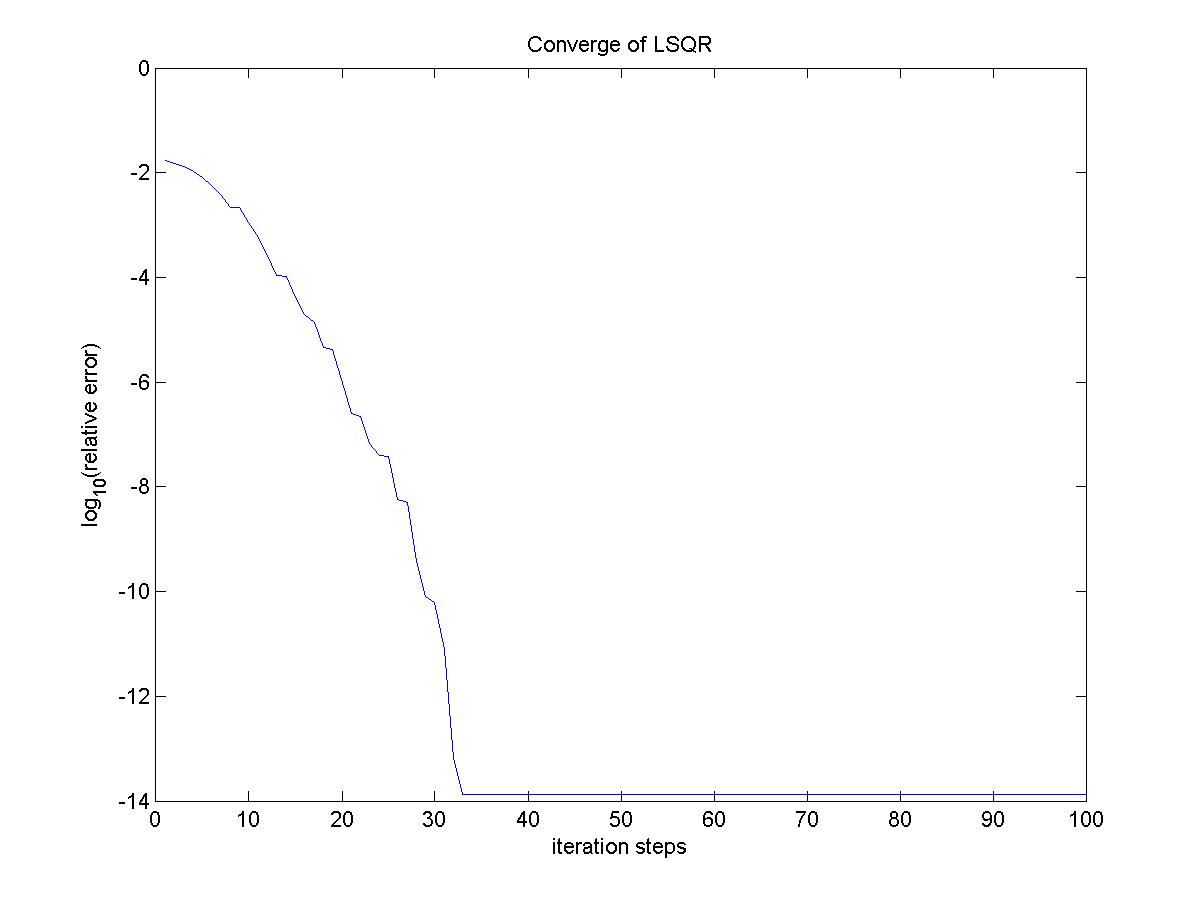
\includegraphics[width=3.5in]{Images/LSQR}
        \end{minipage}
    \end{figure}
\end{frame}


%------------------------------------------------
%------------------------------------------------
% FOURTH SECTION (Nicole's Slides)
%------------------------------------------------
%------------------------------------------------

%\begin{frame}
%\frametitle{Acceleration}
%Since $(I-Q)$ is symmetric positive definite, we accelerate solving: $$(I-Q)x = Tf$$  using the conjugate gradient method.
%
%\end{frame}
%
%%\end{frame}
%\begin{frame}
%\frametitle{Conjugate Gradient Method (Kamath and Sameh, 1988) }
%Step 1 : $x_0 = c$ \\
%\hspace{.5in} Compute $r_0 = Tf - (I-Q)x_0$\\
%\hspace{.5in} Set $p_0 = r_0, i = 0$ \\
%Step 2:  Compute: \\
%\hspace{.5in} $\alpha_i = (r_i, r_i)/(p_i, (I-Q)p_i)$ \\
%\hspace{.5in} $ x_{i+1} = x_i + \alpha_i p_i $ \\
%\hspace{.5in} $\beta_i = (r_{i+1}, r_{i+1})/(r_i, r_i) $ \\
%\hspace{.5in} $p_{i+1} = r_{i+1} + \beta_i p _i $ \\
%Step 3: If convergence criterion is satisfied, terminate the iterations; else set $i = i+1$ and return to Step 2.
%
%\vspace{.4in}
%%We can take a convergence criterion as : $$ \frac{ ||f - A x_i ||}{|| f - A x_0 || } \leq 10^{-6} $$
% We can take a convergence criterion as : $$ \frac{ ||r_i||}{||r_0||} \leq \epsilon$$
%\end{frame}
%
%\begin{frame}
%\frametitle{Conjugate Gradient Method}
%Whenever we see: $$(I - Q) u$$ we really mean to solve multiple least squares problems:
%$$(I-Q) u = (I-P_1)(I-P_2)(I-P_1) u $$
%$$(I-P_i) u \Rightarrow \text{min}_{v} ||u-A_i w|| $$
%\end{frame}
%
%\begin{frame}
%\frametitle{Computing c = Tf}
%
%
%\end{frame}


%\begin{frame}
%frametitle{Distribution of Work}

%\begin{itemize}
%\item \textbf{Wei}: Implement RCM and re-ordering of the matrix, assist my teammates' work
%\item \textbf{Xiaokai}: Parallel Least Squares function, matrix shell function
%\item \textbf{Nate}: CG framework, merge everyone's code together
%\item \textbf{Nicole}: compute c = Tf, MC64 software and ILU preconditioner
%\end{itemize}

%\end{frame}


%%%%%%%%%%%%%%%%
% NEW SLIDES - Comparison/RESULTS
%%%%%%%%%%%%%%%%
\section{Results}

\begin{frame}
\frametitle{Bandsize after Reverse-Cuthill McKee}


\vspace{.2in}

\begin{minipage}{.7\textwidth}
\begin{center}
\begin{tabular}{| l | l | l |}
\hline
matrix             & size        & band size \\
\hline
lns                  & 131         &     32   \\
std1-Jac2-db  & 21,982    &  545  \\
bayer01          & 57,735    &   18,322   \\
venkat25        & 62,424     &  1,515   \\
stomach         & 213,360   &    1,133  \\
atmosmodd    & 1,270,432 &   7,772  \\
\hline
\end{tabular}
\end{center}
\end{minipage}
\begin{minipage}{.29\textwidth}
Bottle-neck - \\ possibly improved by using the Woodbury Formula
\end{minipage}

\end{frame}

%\begin{frame}
%\frametitle{Comparison to ILU Preconditioner}

%For comparison to our parallel solver
% $$ MC64 \, \,  \text{software} + \, \text{GMRES with ILU Preconditioner} $$
% \begin{minipage}{.49\textwidth}
%\begin{figure}[htbp] %  figure placement: here, top, bottom, or page
 %  \centering
 %  \includegraphics[width=3in]{dolphins.png}
%\end{figure}
%\end{minipage}
%\begin{minipage}{.49\textwidth}
%\begin{figure}[htbp] %  figure placement: here, top, bottom, or page
 %  \centering
 %  \includegraphics[width=1.8in]{sparse_matrix.png}
%\end{figure}
%\end{minipage}

%\end{frame}

\begin{frame}
\frametitle{Comparison to ILU Preconditioner}

We re-ordered the matrix first using the MC64 software, then called a Krylov Subspace method with ILU pre-conditioner.
\begin{center}
\begin{tabular}{| l | l | c |}
\hline
matrix             & size        & Converged? \\
\hline
lns                  & 131         &    \color{red} $\times$  \\
std1-Jac2-db  & 21,982    & \color{red}  $\times$  \\
bayer01          & 57,735    &  \color{red} $\times$   \\
venkat25        & 62,424     & \color{green} \Checkmark   \\
stomach         & 213,360   &  \color{green}  \Checkmark  \\
atmosmodd    & 1,270,432 &  \color{green} \Checkmark  \\
\hline


\end{tabular}
\end{center}


\end{frame}



\begin{frame}
\frametitle{tol = $10^{-8}$}
Results for our Krylov Solver is using 4 MPI Processors.
\begin{center}
\begin{tabular}{| l | l | c  c | c  c |}
\hline
                         &                & Our Parallel & Solver & Krylov & ILU\\
                          \hline
    matrix           & size         &    num-its & time (s)     &  num-its & time (s)        \\
 \hline
 lns                   & 131             &     10   &         .1  & \color{red} $\times$  &  \color{red} $\times$\\
 Jac2-db            & 21,982     &    13     &     .8      &  \color{red} $\times$  & \color{red} $\times$ \\
 bayer01        & 57,735  &  \color{red} $\times$    &   \color{red} $\times$    &  \color{red} $\times$  & \color{red} $\times$ \\
 venkat25         & 62,424      & 12     &     1.5   & 374                   & 14.17 \\
 stomach          & 213,360    &   15    & 4 & 16                   & 2.21 \\
 atmosmodd     & 1,270,432 &  14    &  21 &  266                   & 130.72 \\
 \hline

\end{tabular}
\end{center}

\end{frame}

%%%% Some results to show at the very end

\begin{frame}
\frametitle{Runtimes for Smaller Test Cases}
\begin{figure}[htbp] %  figure placement: here, top, bottom, or page
   \centering
   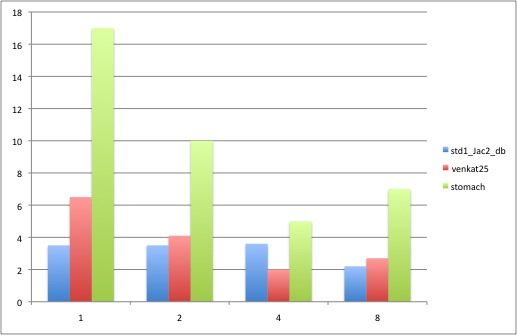
\includegraphics[width=3in]{Images/runtimes.jpg}
   \caption{std1\_Jac2bd: $n = 21982$; venkat25: $n=62424$, stomach: $n=213360$.}
\end{figure}
\end{frame}


\begin{frame}
\frametitle{Runtimes for largest Test Case}
\begin{figure}[htbp] %  figure placement: here, top, bottom, or page
   \centering
   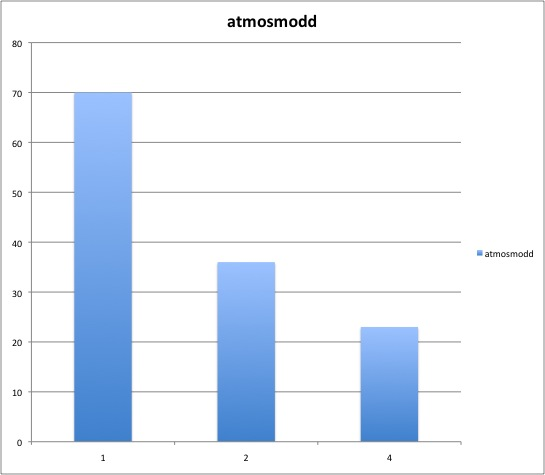
\includegraphics[width=3in]{Images/atmosmodd.jpg}
   \caption{Runtime in seconds for largest test case ($n = 1270432$).}
\end{figure}
\end{frame}


\begin{frame}
\frametitle{References}

[1] Efstratios Gallopoulos, Bernard Philippe, and Ahmed H. Sameh. Pararallelism in Matrix Computations. Springer, 2016.

\vspace{.3in}

[2] Chandrika Kamath and Ahmed Sameh. A projection method for solving nonsymmetric linear systems on multiprocessors. Parallel Computing, 9:291-312, 1988.

\vspace{.3in}

[3] HSL, a collection of Fortran codes for large-scale scientific computation.
    See http://www.hsl.rl.ac.uk/

\end{frame}

\end{document}
